\subsection{Datasets preprocessing}
\subsubsection*{Absenteeism at work Data Set}
The \textit{Absenteeism at work Data Set} is distinct in that it is the only dataset that contains individual records of employees, not just a collective average. This data includes the personal details of the employee, the cause of their absence, and the duration in hours. To ensure the privacy of the subjects, we utilised a Bayesian Network. \\ 
A Bayesian network is a probabilistic graphical model that measures the conditional dependence structure of a set of random variables based on the Bayes theorem. The features that we have used to build the Bayesian network are the \textit{reason for absence}, the \textit{month of absence} and the \textit{absenteeism time}. We added the dependency between \textit{month of absence} and \textit{reason for absence}, since some illnesses are more common during some months of the year, and between \textit{absenteeism time} and \textit{reason for absence}, since based on the type of illness you can request more or less time off (\autoref{fig:bayesian_net}). \\
\begin{figure}[h] 
    \centering
    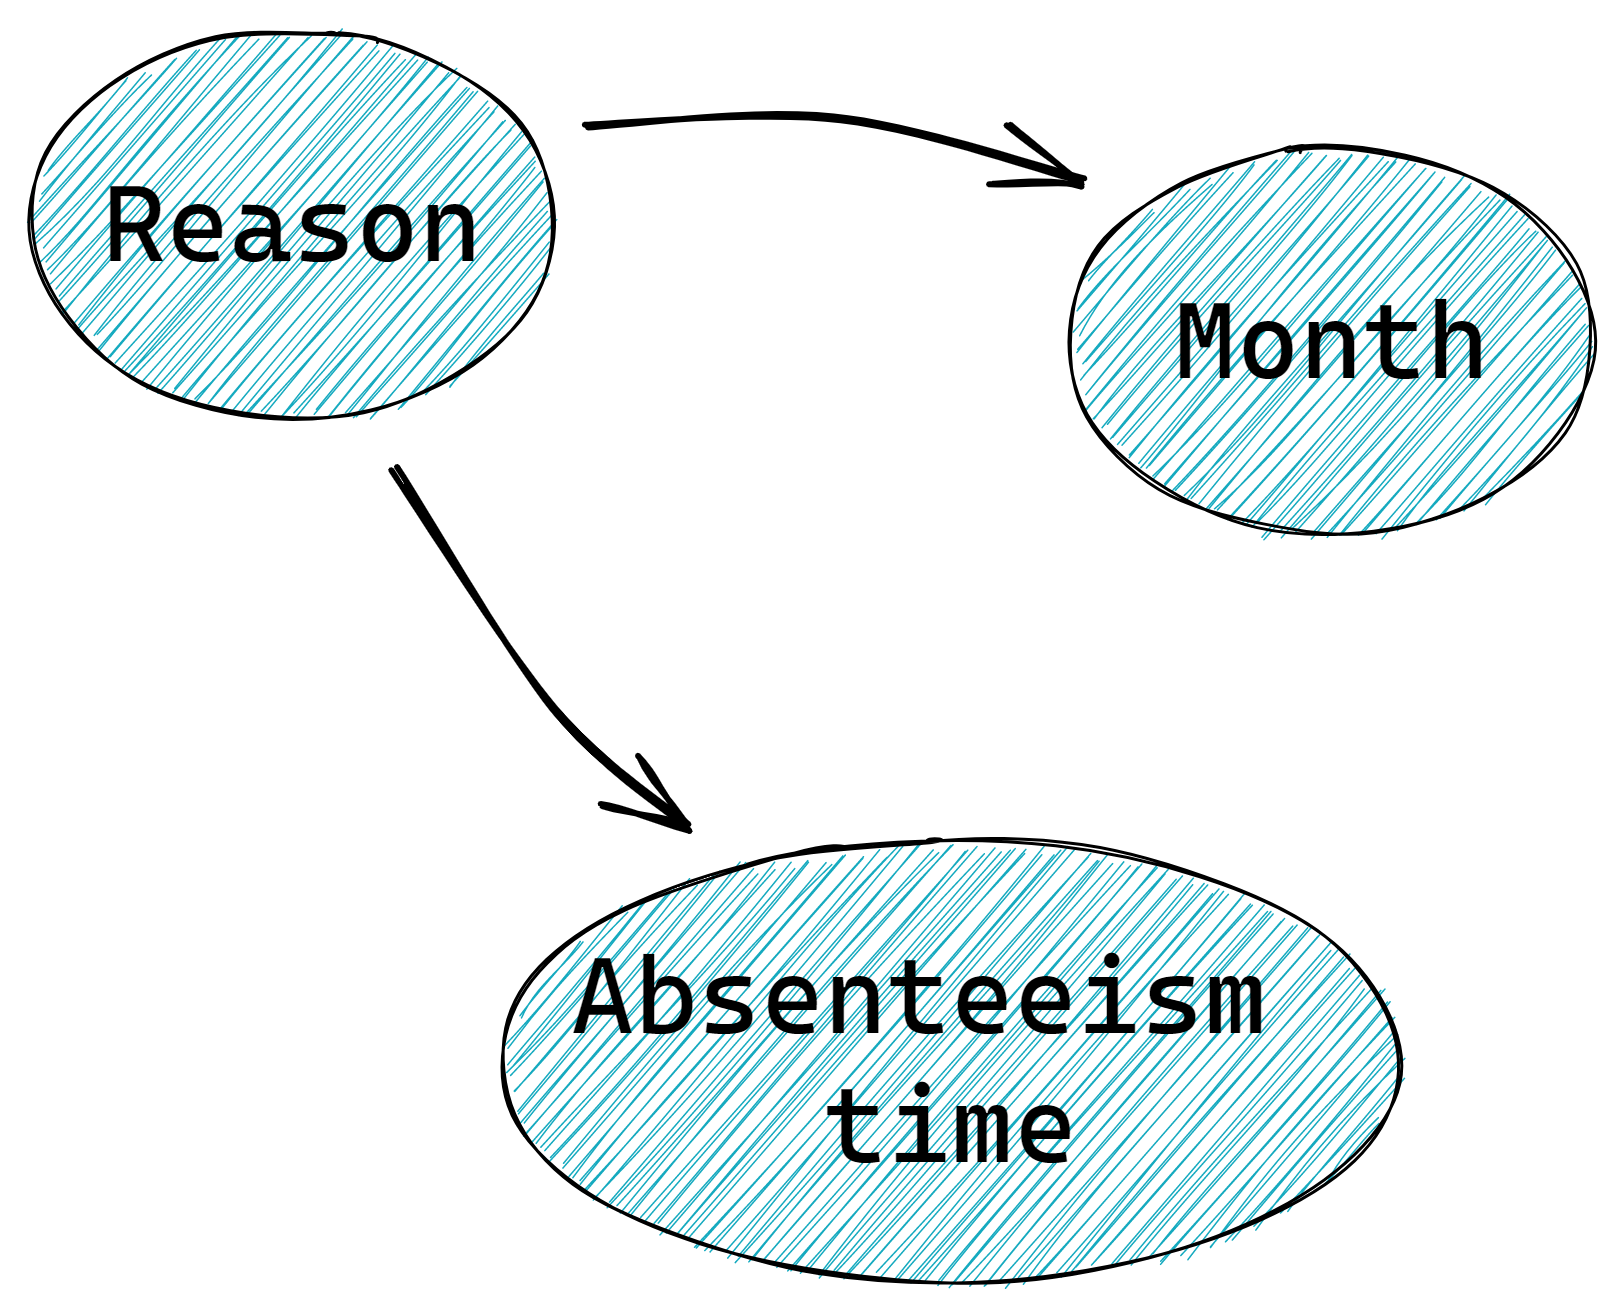
\includegraphics[width=0.5\textwidth]{images/bayesian_net.png}
    \caption{Bayesian network dependencies}
    \label{fig:bayesian_net}
  \end{figure}
Using the \textit{Absenteeism at work Data Set} we learn conditional probability distributions from data, to which we add a Laplace noise for differential privacy. Then we can sample new data that follow the original distributions, but that are not equal to the original ones. \\
The absence reasons in the dataset are given as ICD(International Classification of Diseases) codes, to make them more human-readable, we picked for each ICD code the corresponding more frequent diseases.
\subsubsection*{National Occupational Employment and Wage Estimates United States}
In the \textit{National Occupational Employment and Wage Estimates United States} dataset, we sample employees based on the number of people employed in a certain field. Therefore for example since `Retail Sales Workers` consists of 5.4\% of the total occupations, then the sampled employee will have the 5.4\% of possibility to have as occupation `Retail Sales Worker`. \\
The current salary of the employee is calculated by adding Gaussian noise to the average salary of the employee's occupation, and then the salary raise requested is picked randomly between 5\%-10\%. 
\subsubsection*{Gender pay gap in the UK}
The ranges of the wage gap, used in the tickets regarding the explanation for the gender wage gap in the company, are sampled randomly from the dataset \textit{Gender pay gap in the UK}, adding a Gaussian noise for privacy reasons. 
\subsubsection*{Geonames all cities with a population over 1000}
To sample the cities for the requests of accommodation, we randomly sample from all the cities with more than 100,000 inhabitants from the country of residence of the synthetic employee. To calculate the duration of the accommodation we pick a random number of months between 1 and 12. 
\subsubsection*{OpenFlights database}
To get data for the category type "refund travel", we sample randomly one flight from all the flights leaving from the country of the synthetic employee. The data are taken from the \textit{OpenFlights database}.
\subsubsection*{Complaints - life events}
The complaints about coworkers and superiors and the life events that can affect the work life of a person were written by myself, using primarily personal experience and some help from internet blogs.